\documentclass{article}

\usepackage[italian]{babel}
\usepackage[margin=2cm, footskip=5mm]{geometry}
% questi package non sono necessari in lualatex; ref https://tex.stackexchange.com/a/413046
% \usepackage[utf8]{inputenc}
% \usepackage[T1]{fontenc}
\usepackage{enumitem}
\usepackage{hyperref}
\usepackage{titlesec}
\usepackage{soulutf8}
\usepackage{contour}
\usepackage{float}
\usepackage{graphicx}
\usepackage{fancyhdr}
\usepackage{longtable}
\usepackage[table]{xcolor}
\usepackage{titling}
\usepackage{lastpage}
\usepackage{ifthen}
\usepackage{calc}
\usepackage{minted}
\usepackage{pgfgantt}
\usepackage{subfiles}

\newlength{\imgwidth}

\newcommand\scalegraphics[1]{%
    \settowidth{\imgwidth}{\includegraphics{#1}}%
    \setlength{\imgwidth}{\minof{\imgwidth}{\textwidth}}%
    \includegraphics[width=\imgwidth]{#1}%
}

% XXX definizione dei percorsi in cui cercare immagini
\graphicspath{ {./}
    {./img/}
}

% esempio di utilizzo: \appendToGraphicspath{./img/} (un comando diverso per ogni path da includere)
% N.B.: ci DEVE essere un forward slash alla fine del path, a indicare che è una cartella.
\makeatletter
\newcommand\appendToGraphicspath[1]{%
  \g@addto@macro\Ginput@path{{#1}}%
}
\makeatother

% setup della sottolineatura
\setuldepth{Flat}
\contourlength{0.8pt}

\newcommand{\uline}[1]{%
  \ul{{\phantom{#1}}}%
  \llap{\contour{white}{#1}}%
}

% setup dei link
\hypersetup{
  colorlinks=true, % set true if you want colored links
  linktoc=all,     % set to all if you want both sections and subsections linked
  linkcolor=black, % choose some color if you want links to stand out
}

% setup di header e footer
\pagestyle{fancy}

\fancyhf{}
\fancyhead[L]{\includegraphics[width=1cm]{logo.png}}
\fancyhead[R]{\thetitle}
\fancyfoot[R]{\thepage\ di~\pageref{LastPage}}

\fancypagestyle{nopage}{%
  \fancyfoot{}%
}

\setlength{\headheight}{1.2cm}

% setup forma \paragraph e \subparagraph
\titleformat{\paragraph}[hang]{\normalfont\normalsize\bfseries}{\theparagraph}{1em}{}
\titleformat{\subparagraph}[hang]{\normalfont\normalsize\bfseries}{\thesubparagraph}{1em}{}

% setup profondità indice di default
\setcounter{secnumdepth}{5}
\setcounter{tocdepth}{5}

% shortcut per i placeholder
\newcommand{\plchold}[1]{\textit{\{#1\}}} % chktex 20

% hook per lo script che genera il glossario
\newcommand{\glossario}[1]{\underline{#1}\textsubscript{g}}

% definizione dei comandi \uso e \stato
\makeatletter
\newcommand{\setUso}[1]{%
  \newcommand{\@uso}{#1}%
}
\newcommand{\uso}{\@uso}

\newcommand{\setStato}[1]{%
  \newcommand{\@stato}{#1}%
}
\newcommand{\stato}{\@stato}

\newcommand{\setVersione}[1]{%
  \newcommand{\@versione}{#1}%
}
\newcommand{\versione}{\@versione}

\newcommand{\setResponsabile}[1]{%
  \newcommand{\@responsabile}{#1}%
}
\newcommand{\responsabile}{\@responsabile}

\newcommand{\setRedattori}[1]{%
  \newcommand{\@redattori}{#1}%
}
\newcommand{\redattori}{\@redattori}

\newcommand{\setVerificatori}[1]{%
  \newcommand{\@verificatori}{#1}%
}
\newcommand{\verificatori}{\@verificatori}

\newcommand{\setDescrizione}[1]{%
  \newcommand{\@descrizione}{#1}%
}
\newcommand{\descrizione}{\@descrizione}

\newcommand{\setModifiche}[1]{%
  \newcommand{\@modifiche}{#1}%
}

\newcommand{\modifiche}{\@modifiche}

\makeatother

% setup delle description
\setlist[description,1]{font=$\bullet$\hspace{1.5mm}, labelwidth=* leftmargin=*,labelindent=12.5mm}
\setlist[description,2]{font=$\bullet$\hspace{1.5mm}, leftmargin=*,labelindent=12.5mm}

\appendToGraphicspath{../../commons/img/}

\title{Verbale esterno --- 05/05/2020}

\setResponsabile{Luca Ercole}
\setRedattori{Alberto Gobbo}
\setVerificatori{
  Alberto Cocco
}
\setUso{Esterno}
\setDescrizione{Verbale dell'incontro di GruppOne del 05/05/2020}
\setModifiche{%
\cellcolor{white!80!lightgray!100} & Luca Ercole & 2020--05--06 & approva documento \\%
\cellcolor{white!80!lightgray!100} & Alberto Cocco & 2020--05--05 & verifica verbale \\%
\multirow{-3}{*}{-} & Alberto Gobbo & 2020--05--05 & stendi verbale%
}

\disabilitaVersione{}
\disabilitaElencoFigure{}
\disabilitaElencoTabelle{}

\begin{document}

\thispagestyle{empty}
\pagenumbering{gobble}

\begin{center}

  \includegraphics[width=8.5cm]{\commons/img/logo.png}\\
  {\Large GruppOne - progetto "Stalker"}\\
  \vspace{1.5cm}

  {\Huge \thetitle}
  \vspace{1.5cm}

  \begin{table}[H]
    \centering

    \begin{tabular}{r|l}
      \textbf{Versione}     & \versione              \\
      \textbf{Approvazione} & \responsabile          \\
      \textbf{Redazione}    & \redattori             \\
      \textbf{Verifica}     & \verificatori          \\
      \textbf{Stato}        & \stato                 \\
      \textbf{Uso}          & \uso                   \\
      \textbf{Destinato a}  & Imola Informatica      \\
                            & GruppOne               \\
                            & Prof. Tullio Vardanega \\
                            & Prof. Riccardo Cardin  \\
    \end{tabular}
  \end{table}

  \vspace{3cm}
  \textbf{Descrizione}\\
  \descrizione\\
  \vfill
  \verb|gruppone.swe@gmail.com|
\end{center}

\newpage
\thispagestyle{nopage}

\section*{Registro delle modifiche}
\label{sec:registro_delle_modifiche}

\begin{table}[H]
  \label{tab:registro_delle_modifiche}

  \centering
  \rowcolors{2}{lightgray}{white!80!lightgray!100}

  \begin{longtable}[c]{c c c c l}
    \rowcolor{darkgray!90!}\color{white}{\textbf{Versione}} & \color{white}{\textbf{Data}} & \color{white}{\textbf{Nominativo}} & \color{white}{\textbf{Ruolo}} & \color{white}{\textbf{Descrizione}} \\\endhead
    \modifiche
  \end{longtable}
\end{table}

% section registro_delle_modifiche (end)
\newpage

\thispagestyle{nopage}
\pagenumbering{roman}
\tableofcontents

\newpage

\pagenumbering{arabic}


\section{Informazioni logistiche}%
\label{sec:informazioni_logistiche}

\begin{description}
  \item [Luogo] chiamata Zoom
  \item [Data] 05/05/2020
  \item [Ora] 13:40 \symbol{8594} 14:00
\end{description}

\subsection{Membri del gruppo presenti}%
\label{sub:membri_del_gruppo_presenti}

\begin{enumerate}
  % \item Riccardo Agatea
  % \item Tobia Apolloni
  % \item Riccardo Cestaro
  % \item Alberto Cocco
  \item Luca Ercole
  \item Alberto Gobbo
  \item Alessandro Rizzo
  \item Fabio Scettro
\end{enumerate}
% sub:membri_del_gruppo_presenti (end)

\subsection{Altri partecipanti}%
\label{sub:altri_partecipanti}

\begin{enumerate}
  \item Prof.\ Riccardo Cardin (committente)
\end{enumerate}

\section{Introduzione}%
\label{sec:introduzione}

L'incontro, avvenuto tramite chiamata sulla piattaforma Zoom, ci è servito per chiarire i dubbi riguardanti lo sviluppo dei diagrammi delle classi da inserire nell'allegato tecnico che consegneremo al Prof.Cardin in data 08/05/2020.

\section{Ordine del giorno}%
\label{sec:ordine_del_giorno}

\begin{itemize}
  \item Struttura e contenuto dell'allegato tecnico
  \item Specifica API nell'allegato tecnico
  \item Utilizzo specifica TypeScript nella specifica UML
  \item Interpretazione UML dell'implementazione anonima di un'interfaccia
  \item Constructor Injection di Angular in UML
  \item Interpretazione UML delle interfacce repository
  \item Dichiarazione interfacce di framework in UML
\end{itemize}

\section{Struttura e contenuto dell'allegato tecnico}%
\label{sec:struttura_e_contenuto_allegato_tecnico}

\textbf{Domanda:} Noi pensavamo di fornirle un documento contenente una serie di diagrammi (tra i più corposi cha abbiamo sviluppato) con annessa descrizione, suddivisi per componente e per feature (per una visione generale del funzionamento dei componenti). In particolare, vorremmo fornirle i diagrammi delle classi dettagliati per ogni componente che abbiamo usato, e i diagrammi di sequenza solo dove lo riteniamo necessario. C'è qualcos'altro che va aggiunto all'allegato tecnico? È una struttura accettabile?

\textbf{Risposta:} Mi sembra una struttura accettabile. Le informazioni che avete specificato voi sono quelle sufficienti per avere un quadro generale della vostra architettura.

\section{Specifica API nell'allegato tecnico}%
\label{sec:specifica_api_allegato_tecnico}

\textbf{Domanda:} La comunicazione tra componenti la stiamo regolamentando attraverso un contratto definito mediante una specifica API, ma non ci siamo preoccupati di renderla esplorabile. Può essere comunque di suo interesse se le passassimo la specifica e i modelli in JSON, oppure direttamente il file openapi.yaml?

\textbf{Risposta:} Se riuscite a inserire i modelli nel documento, può andare bene. Ma potete comunque allegarmi il vostro file nell'allegato tecnico.

\section{Utilizzo specifica TypeScript nella specifica UML}%
\label{sec:utilizzo_specifica_typescript_in_specifica_uml}

\textbf{Domanda:} Abbiamo delle domande specifiche sui diagrammi per la web application che stiamo sviluppando in \textit{Angular}, che sono diagrammi che si convertono in TypeScript. Per rispettare la specifica API definita, in alcuni diagrammi abbiamo dei campi facoltativi che su TypeScript vengono definiti con \textbf{?}, che equivalgono alla voce \textit{undefined}. È una definizione corretta, oppure ci dobbiamo attenere alla specifica UML, che impone di definire il valore che assumono le variabili?

\textbf{Risposta:} Se non utilizzi una specifica UML, il diagramma che stai sviluppando non è più un diagramma UML, oppure se la stai utilizzando vuol dire che stai sviluppando un diagramma non conforme alla specifica. La specifica è come un linguaggio, in quanto ha le sue regole che devono essere rispettate. Il vincolo \textbf{?} non può essere inserito nella specifica UML, quindi va eliminato. Ci potrebbe essere un modo alternativo utilizzando le proprietà aggiuntive dei singoli campi, ma bisogna vedere se questo porta valore aggiunto al diagramma. In ogni caso, quello che state cercando di implementare è molto dettagliato (\textit{overkill}), quindi potete tranquillamente eliminarlo.

\section{Interpretazione UML dell'implementazione anonima di un'interfaccia}%
\label{sec:Interpretazione_uml_implementazione_anonima_interfaccia}

\textbf{Domanda:} TypeScript permette di istanziare un oggetto su un'implementazione anonima (cioè non le fornisco un nome perchè non la utilizzo in altre parti del codice) di un'interfaccia esistente. In questo caso, come devo interpretare l'interfaccia rispettando la specifica UML\%?

\textbf{Risposta:} Per essere rigorosi, si dovrebbe dare sia l'interfaccia che l'implementazione che fornisci. Nulla ti vieta di trovare un modo per specificare che quell'implementazione è anonima, ma non è obbligatorio e quindi puoi anche farne a meno.

\section{Constructor Injection di Angular in UML}%
\label{sec:constructor_injection_angular_uml}

\textbf{Domanda:} In Angular viene utilizzata la Constructor Injection, principalmente nei \textit{services} e nei \textit{components}, per passare altri servizi o altri componenti come se fossero parametri effettivi della classe. Nel diagramma UML, noi li abbiamo dichiarati come parametri effettivi della classe che sono dichiarati solamente nel costruttore del \textit{component} o del \textit{service}. È corretto?

\textbf{Risposta:} Sì, è corretto. Fate comunque attenzione che la sintassi dei linguaggi Object-Oriented e la sua rappresentazione in UML concettualmente sono distanti. Quando dichiari il costruttore, automaticamente dici quali sono gli attributi della classe.

\section{Interpretazione UML delle interfacce repository}%
\label{sec:interpretazione_uml_interfacce_repository}

\textbf{Domanda:} Abbiamo un paio di domande riguardo al server. Il driver e il framework Spring (per l'interfaccia con i repository) che stiamo utilizzando, ci permette di utilizzare delle interfacce invece che delle classi per definire i repository. Noi stiamo utilizzando il driver \textit{R2DBC}, un driver asincrono reattivo per connettersi ai database SQL, e i nostri repository sono semplicemente delle interfacce che estendono l'interfaccia \textit{ReactiveCrudRepository} fornita da Spring. Il problema sorge dal fatto che non ci sia una classe dichiarata che implementi l'interfaccia. Come possiamo descrivere questo particolare nei diagrammi UML\%?

\textbf{Risposta:} Inserite l'interfaccia in modo classico, inserendo solo i metodi che state utilizzando di quell'interfaccia e quelli che vengono definiti da voi.

\section{Dichiarazione interfacce di framework in UML}%
\label{sec:dichiarazione_interfacce_framework_uml}

\textbf{Domanda:} Se un'interfaccia estende un'altra interfaccia definita da Spring, noi non dobbiamo preoccuparci di implementarla nel diagramma UML\%?

\textbf{Risposta:} Sarebbe bene che voi mettiate i tipi di frontiera del framework che utilizzate. Ovviamente vanno scritti \textbf{fuori} dai vostri package, in quanto non è un'interfaccia creata appositamente da voi, ma da Spring.

\newpage
\section{Registro delle decisioni}%
\label{sec:registro_delle_decisioni}

\begin{description}
  \item[20200505-ext-001] Il gruppo ha deciso di mantenere la struttura e il contenuto attuale dell'allegato tecnico, in quanto ritenuta soddisfacente dal committente.
  \item[20200505-ext-002] Il gruppo ha deciso di allegare la specifica API all'allegato tecnico.
  \item[20200505-ext-003] Il gruppo ha deciso di uniformare tutti i diagrammi alla specifica UML\@.
\end{description}

% sec:registro_delle_decisioni (end)
\end{document}
